\documentclass[tikz,border=8pt]{standalone}
\usepackage{amsmath,amssymb}
\usetikzlibrary{arrows.meta,automata,positioning,quotes}
\begin{document}
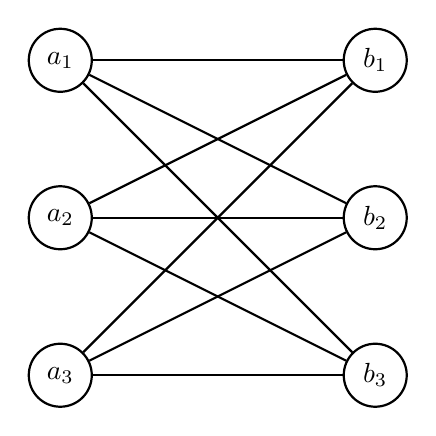
\begin{tikzpicture}[x=1cm,y=1cm]
\tikzset{
  graphnode/.style={circle,draw,thick,minimum size=8mm,inner sep=1pt,font=\sffamily},
  directed/.style={-{Stealth[length=2.4mm]},thick},
  undirected/.style={thick}
}
\node[graphnode] (n_a1) at (0.00,2.00) {$a_1$};
\node[graphnode] (n_a2) at (0.00,0.00) {$a_2$};
\node[graphnode] (n_a3) at (0.00,-2.00) {$a_3$};
\node[graphnode] (n_b1) at (4.00,2.00) {$b_1$};
\node[graphnode] (n_b2) at (4.00,0.00) {$b_2$};
\node[graphnode] (n_b3) at (4.00,-2.00) {$b_3$};
\draw[undirected] (n_a1) -- (n_b1);
\draw[undirected] (n_a1) -- (n_b2);
\draw[undirected] (n_a1) -- (n_b3);
\draw[undirected] (n_a2) -- (n_b1);
\draw[undirected] (n_a2) -- (n_b2);
\draw[undirected] (n_a2) -- (n_b3);
\draw[undirected] (n_a3) -- (n_b1);
\draw[undirected] (n_a3) -- (n_b2);
\draw[undirected] (n_a3) -- (n_b3);
\end{tikzpicture}
\end{document}
